\section{Модель сухого электронно-лучевого травления резиста.}

Вышеописанные модели отдельных процессов, протекающих при сухом электронно-лучевом травлении резиста, были объединены в алгоритме моделирования конечного профиля линии, получаемой методом СЭЛТР. В этом алгоритме все время экспонирования разбивалось на промежутки величиной 1~с, и в течение каждого промежутка последовательно производились следующие действия:

\begin{enumerate}
	\item Моделирование рассеяния электронного пучка в ПММА и подложке;
	\item Моделирование электронно-стимулированных разрывов молекул \linebreak ПММА;
	\item Вычисление локальной молекулярной массы и вязкости ПММА;
	\item Вычисление объемов образовавшихся в ПММА микрополостей;
	\item Преобразование слоя ПММА со внутренними микрополостями в пилообразную структуру;
	\item Моделирование растекания пилообразной структуры;
	\item Определение нового положение вершин поверхности слоя ПММА.
\end{enumerate}

По истечении всего времени экспонирования также моделировалось растекание слоя ПММА при его охлаждения до температуры, при которой процессы растекания перестают протекать заметным образом (было установлено, что эта температура составляет около 80 $^\circ$C).

Демонстрация процесса моделирования профиля линии, получаемой методом СЭЛТР, приведена на рисунке~\ref{fig:DEBER_example}. Моделирование проводилось для следующих условий условий процесса СЭЛТР: начальная толщина слоя ПММА равна 500~нм, энергия электронного пучка $E$ = 20 кэВ, температура образца $T$~=~150~$^{\circ}$C/c, время экспонирования $t_\mathrm{exp}$ = 100 с, плотность тока экспонирования на единицу длины $j_\mathrm{l}$ = 10 пА/см, скорость охлаждения образца после экспонирования составляла 1~$^{\circ}$C/с.

\begin{figure}[t!]
	\begin{minipage}{0.48\textwidth}
		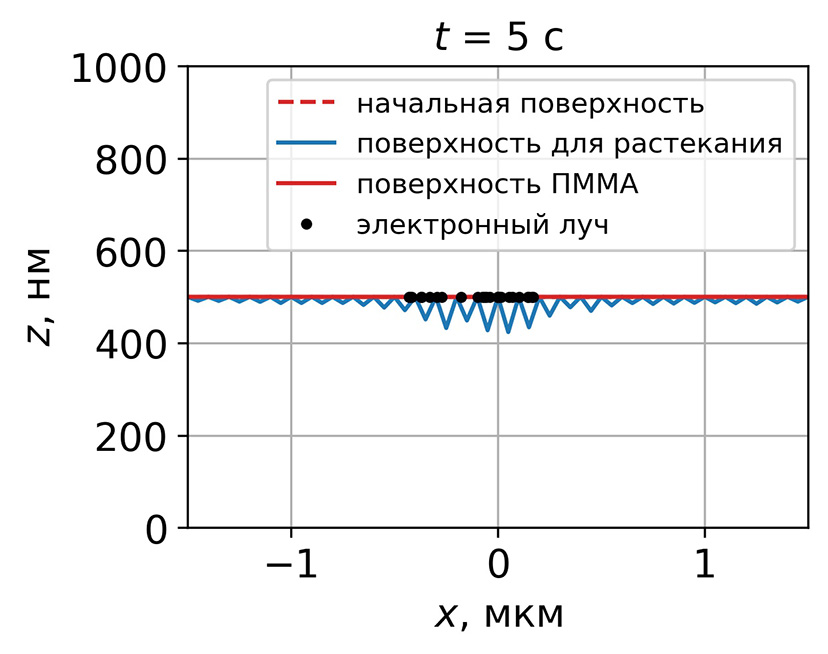
\includegraphics[width=\linewidth]{DEBER_example/example_5_200} \\
		\vspace{-13em} \\ \text{\hspace{0em} a}) \\ \vspace{13em}
	\end{minipage}
	\begin{minipage}{0.48\textwidth}
		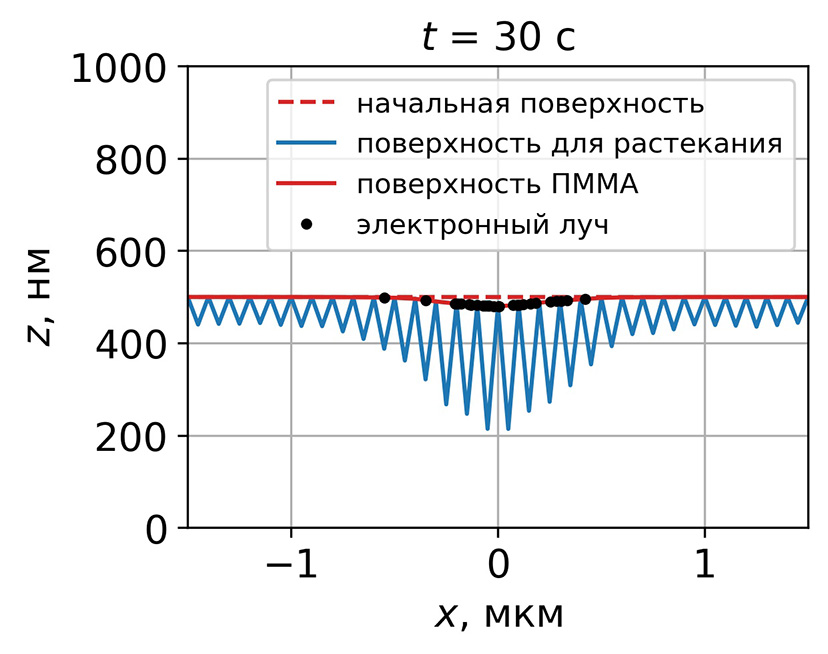
\includegraphics[width=\linewidth]{DEBER_example/example_30_200} \\
		\vspace{-13em} \\ \text{\hspace{-0.1em} б}) \\ \vspace{13em}
	\end{minipage}
	
	\vspace{-3em}
	
	\begin{minipage}{0.48\textwidth}
		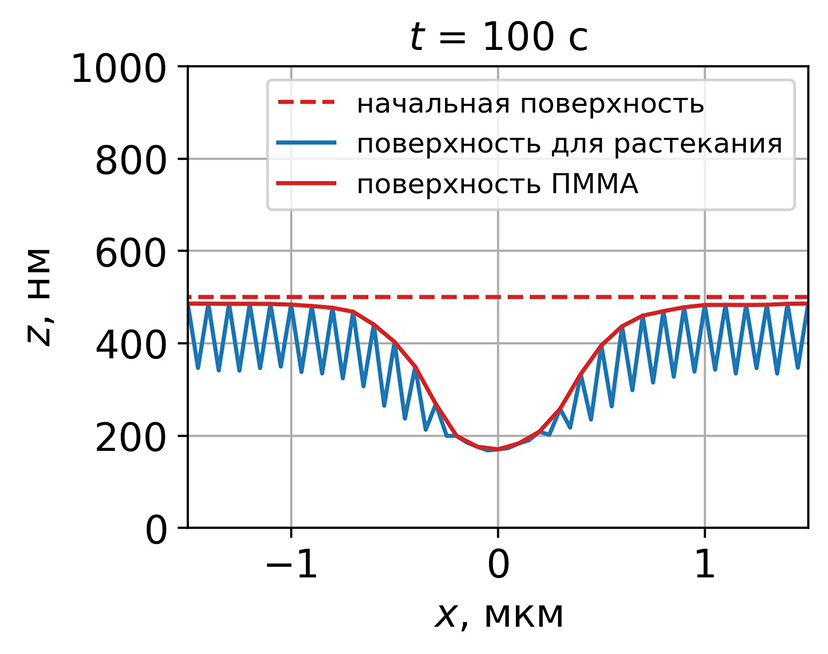
\includegraphics[width=\linewidth]{DEBER_example/example_100_200} \\
		\vspace{-13em} \\ \text{\hspace{0em} в}) \\ \vspace{13em}
	\end{minipage}
	\begin{minipage}{0.48\textwidth}
		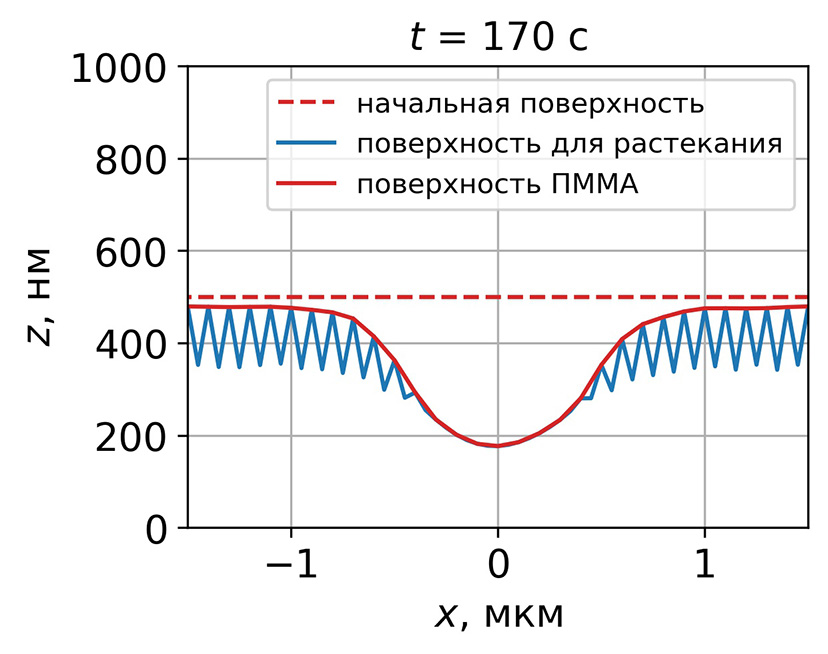
\includegraphics[width=\linewidth]{DEBER_example/example_170_200} \\
		\vspace{-13em} \\ \text{\hspace{-0.1em} г}) \\ \vspace{13em}
	\end{minipage}
	\vspace{-3em}
	\caption{Моделирование профиля линии, получаемой методом СЭЛТР, в различные моменты времени в течение процесса экспонирования и охлаждения образца. Условия экспонирования: $E$ = 20 кэВ, $T$ = 150 $^{\circ}$C/c, $t_\mathrm{exp}$ = 100 с, плотность тока экспонирования на единицу длины $j_\mathrm{l}$ = 10 пА/см, скорость охлаждения образца -- 1~$^{\circ}$C/с. Красная пунктирная линия обозначает начальное положение поверхности слоя ПММА, черные точки -- координаты точек входа электронного пучка в слой резиста.}
	\label{fig:DEBER_example}
\end{figure}

На основе моделирования процесса СЭЛТР можно сделать следующие общие заключения о процессе формирования линии в данном процессе. В начальные моменты времени экспонирование резиста приводит к его деполимеризации и появлению в нем микрополостей, однако, процессы растекания еще не могут протекать заметным образом за счет большой вязкости резиста (рисунок~\ref{fig:DEBER_example},~a)). При дальнейшем экспонировании молекулярная масса и, соответственно, вязкость резиста снижаются до значений, при которых становится возможным заметное растекание резиста и заполнение микрополостей (рисунок~\ref{fig:DEBER_example},~б)). С этого момента времени процессы деполимеризации резиста, уменьшения его вязкости, образования новых микрополостей и заполнения старых протекают одновременно до окончания экспонирования. При окончании экспонирования прекращается образование новых микрополостей и уменьшение вязкости резиста, и дальнейшее охлаждение образца сопровождается только заполнением существующих микрополостей (рисунок~\ref{fig:DEBER_example}, в)). С уменьшением температуры образца вязкость резиста увеличивается, и процессы растекания затухают (рисунок~\ref{fig:DEBER_example}, г)).

